\documentclass{article}
\usepackage{graphicx} % Required for inserting images
\usepackage{float}

\title{Swetify}
\author{Niccolò Malgeri, Filippo Viti, Alessio Delli Colli}
\date{July 2024}

\begin{document}

\maketitle

\tableofcontents
\newpage


\section{Motivazioni}
Il nostro intensivo utilizzo di piattaforme di streaming musicali ha suscitato in noi un interesse riguardo
la loro struttura e il desiderio di replicarne il funzionamento.\\
Abbiamo deciso quindi di realizzare un'applicazione che simuli le loro funzionalità da noi denominata Swetify.
\section{Requisiti Funzionali}
Swetify prevede la partecipazione di due tipologie di utenti: cliente e artista.

\subsection{Funzionalità proposte al cliente}

\begin{itemize}
\item
  visualizzare un catalogo musicale che consenta agli utenti di cercare brani, album e artisti tramite una barra
  di ricerca.
  
\item
  visualizzare le informazioni dettagliate di un brano, inclusi titolo, artista, album e durata.
  
\item
  riprodurre, mettere in pausa e saltare i brani.

\item
  creare, modificare ed eliminare le proprie playlist, aggiungere e rimuovere brani da queste playlist.

\item
  ricevere raccomandazioni di brani basate sulla cronologia di ascolto dell'utente

\item
  seguire gli artisti per ricevere aggiornamenti sui nuovi rilasci.
  
\end{itemize}

\subsection{Funzionalità proposte all'artista}

\begin{itemize}
\item
  caricare album contenenti canzoni o podcast.
\end{itemize}

\subsection{Diagramma dei casi d'uso}
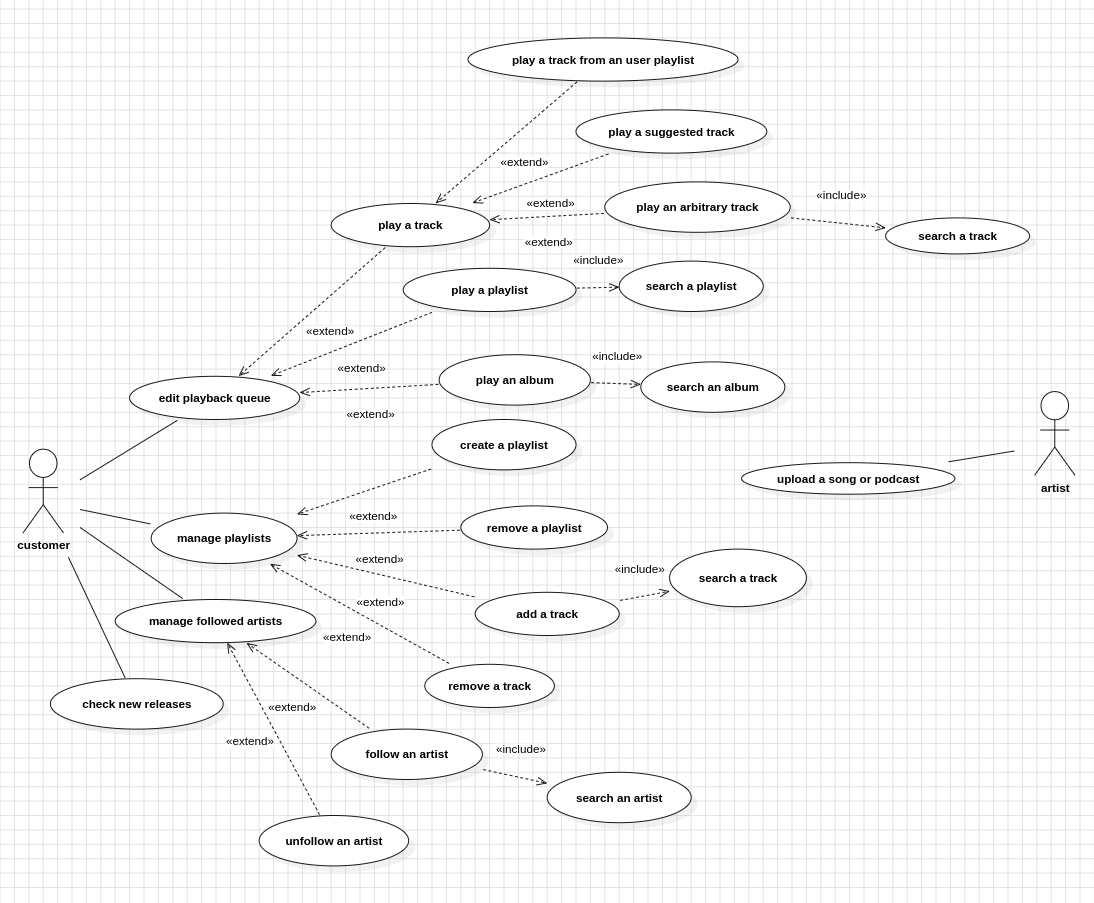
\includegraphics[scale=0.33]{usecase04}

\subsection{Template dei casi d'uso}



\begin{center}
\begin{tabular}{|l|l|}
  \hline
  \textbf{UC1} & \textbf{riproduzione canzone}\\
  \hline
    livello & user goal\\
  \hline
    descrizione & l'utente cerca e riproduce una canzone\\
  \hline
    attori & cliente\\
  \hline
    pre-condizioni & l'utente deve avere le credenziali per effettuare l'accesso\\
  \hline
    post-condizioni & la canzone selezionata viene aggiunta alla coda\\
  \hline
  normale svolgimento & 1) l'utente apre la pagina di ricerca\\
                      & 2) inserisce il nome di una canzone\\
                      & 3) seleziona una voce dall'elenco proposto\\
                      & 4) seleziona l'opzione ``aggiungi in coda"
                        
  \\
  \hline
    svolgimenti alternativi & 4b) l'utente seleziona l'opzione "aggiungi in testa"\\
  \hline
  
\end{tabular}

\vspace{40pt}

\begin{tabular}{|l|l|}
  \hline
  \textbf{UC2} & \textbf{modifica playlist}\\
  \hline
    livello & user goal\\
  \hline
    descrizione & l'utente modifica una delle sue playlist personali\\
  \hline
    attori & cliente\\
  \hline
  pre-condizioni & l'utente deve avere le credenziali per effettuare l'accesso\\
  &ed avere una playlist salvata\\
  \hline
    post-condizioni & la playlist presenta i cambiamenti apportati dall'utente\\
  \hline
  normale svolgimento & 1) l'utente apre la pagina "le mie playlist"\\
                      & 2) l'utente seleziona la playlist da modificare\\
                      & 3) l'utente cerca una canzone da aggiungere\\
                      & 4) l'utente termina salvando le modifiche

  \\
  \hline
  svolgimenti alternativi & 3b) l'utente seleziona una canzone da rimuovere\\
                          & 4b) l'utente annulla le modifiche alla playlist\\
  \hline
  
\end{tabular}

\vspace{40pt}

\begin{tabular}{|l|l|}
  \hline
  \textbf{UC3} & \textbf{aggiunta album}\\
  \hline
    livello & user goal\\
  \hline
    descrizione & l'artista carica un nuovo album sul suo profilo\\
  \hline
    attori & artista\\
  \hline
    pre-condizioni & l'artista deve avere le credenziali per effettuare l'accesso\\
  \hline
    post-condizioni & il nuovo album è visibile se cercato dagli utenti\\
  \hline
  normale svolgimento & 1) l'artista seleziona l'opzione carica album\\
                      & 2) inserisce i nomi delle canzoni ed i rispettivi dati\\
                      & 3) l'artista termina l'inserimento salvando l'album
  \\
  \hline
    svolgimenti alternativi & 3b) l'artista annulla il caricamento dell'album\\
  \hline
  
\end{tabular}

\vspace{40pt}

\begin{tabular}{|l|l|}
  \hline
  \textbf{UC4} & \textbf{iscrizione ad un artista}\\
  \hline
    livello & user goal\\
  \hline
    descrizione & l'utente aggiunge un artista agli artisti seguiti\\
  \hline
    attori & cliente\\
  \hline
  pre-condizioni & l'utente deve avere le credenziali per effettuare l'accesso\\
  \hline
  post-condizioni & nel momento in cui l'artista carica un nuovo album\\
                  & l'utente può visualizzarlo nella sezione\\
                  & "nuovi rilasci"\\
  \hline
  normale svolgimento \hspace{5pt} & 1) l'utente apre la pagina di ricerca\\
                      & 2) inserisce il nome di una canzone\\
                      & 3) seleziona una voce dall'elenco proposto\\
                      & 4) seleziona l'opzione ``aggiungi in coda"
  \\
  \hline

  
\end{tabular}
\end{center}

\newpage

\subsection{Mockups}
\subsubsection{Pagina di accesso}
\begin{figure}[H]
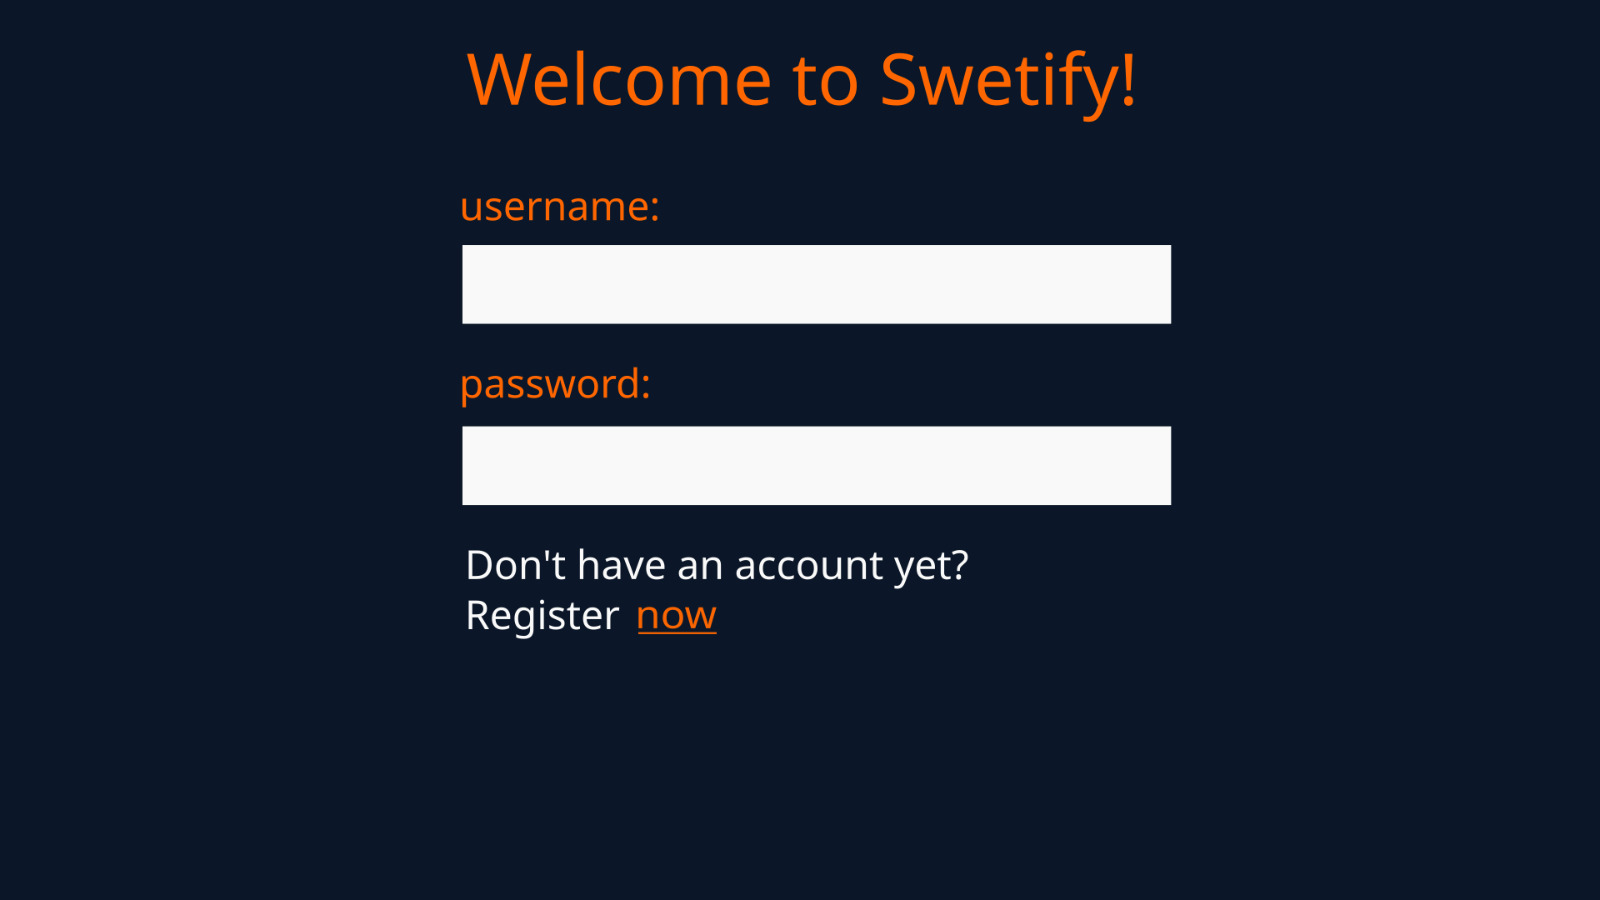
\includegraphics[scale=0.25]{welcome}
\end{figure}
\subsubsection{Pagina di ricerca}
\begin{figure}[H]
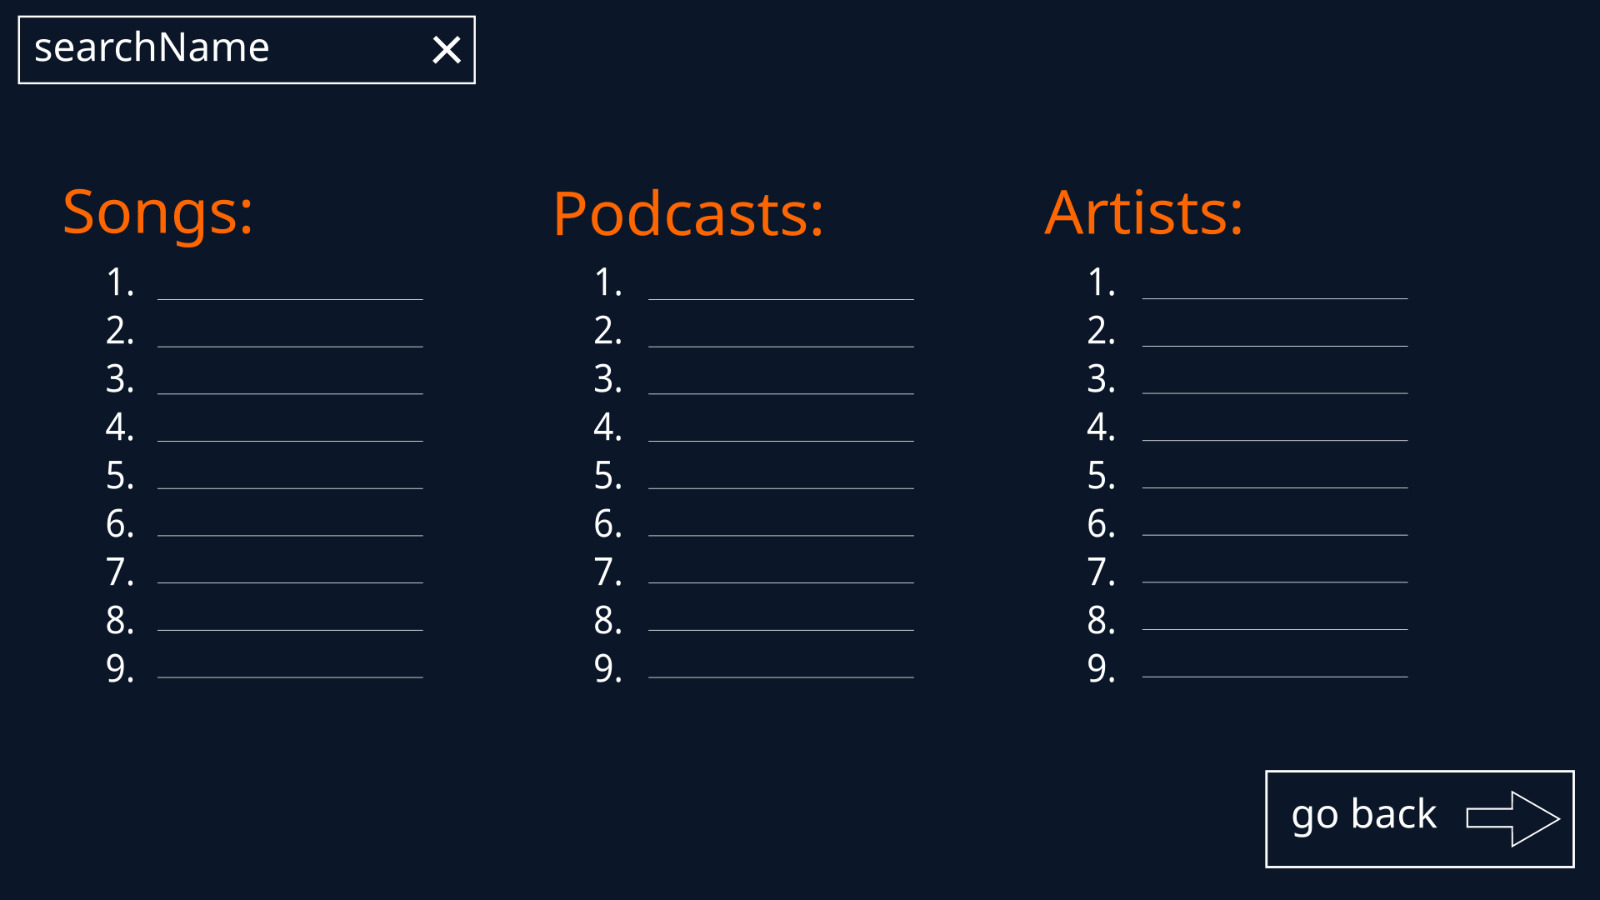
\includegraphics[scale=0.25]{search}
\end{figure}
\subsubsection{Suggerimenti}
\begin{figure}[H]
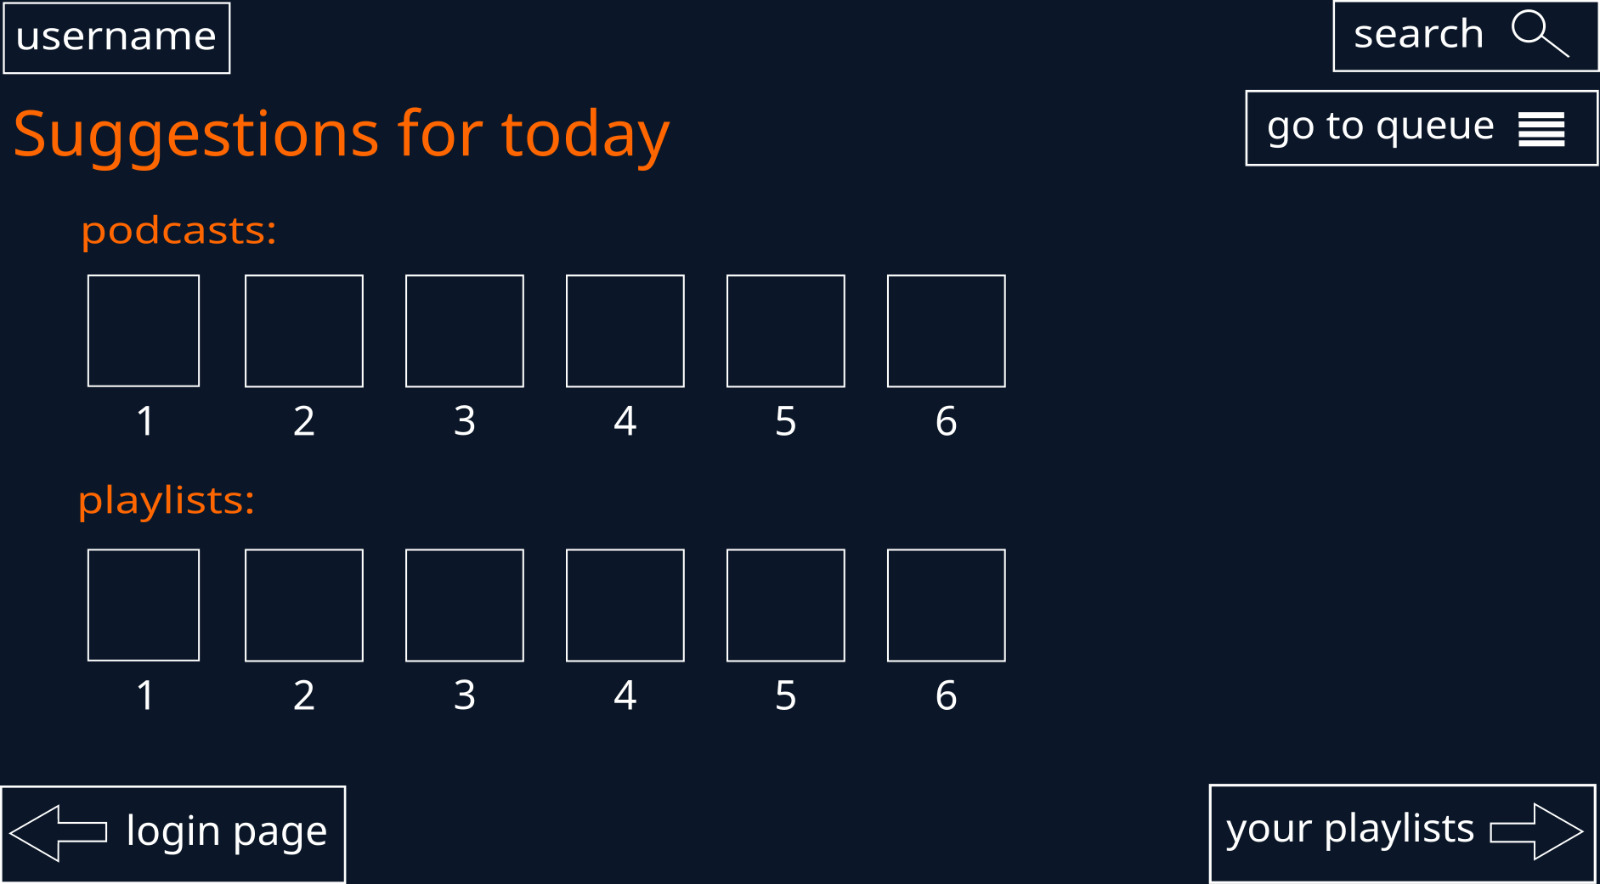
\includegraphics[scale=0.25]{suggestions}
\end{figure}
\subsubsection{Coda di riproduzione}
\begin{figure}[H]
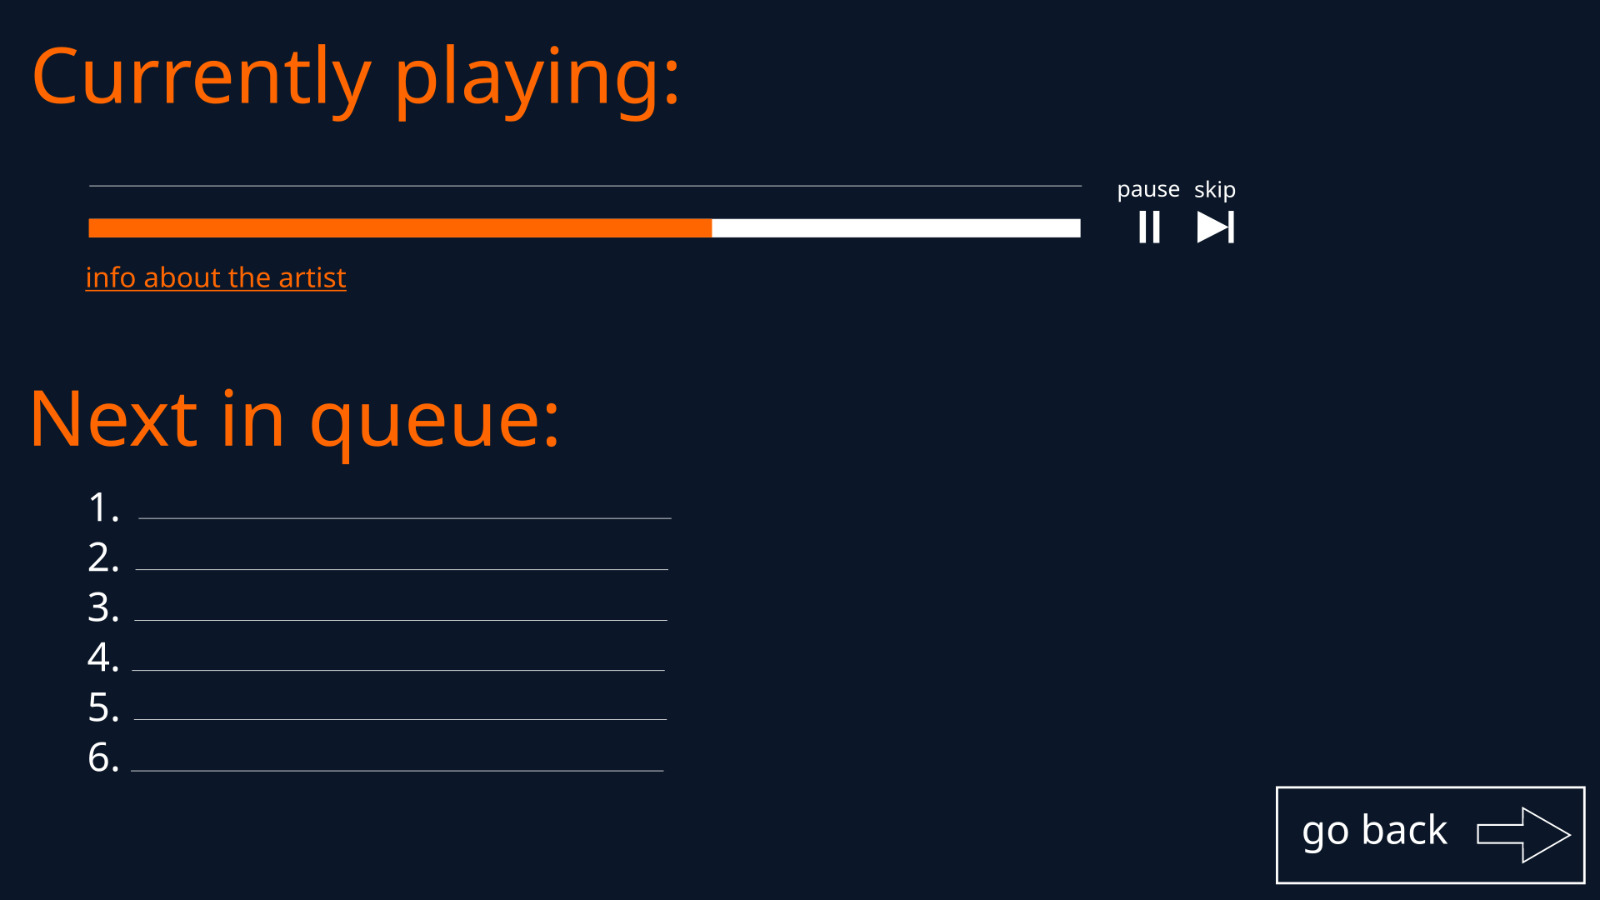
\includegraphics[scale=0.25]{playback}
\end{figure}

\subsection{Sequence diagram}
\begin{figure}[H]
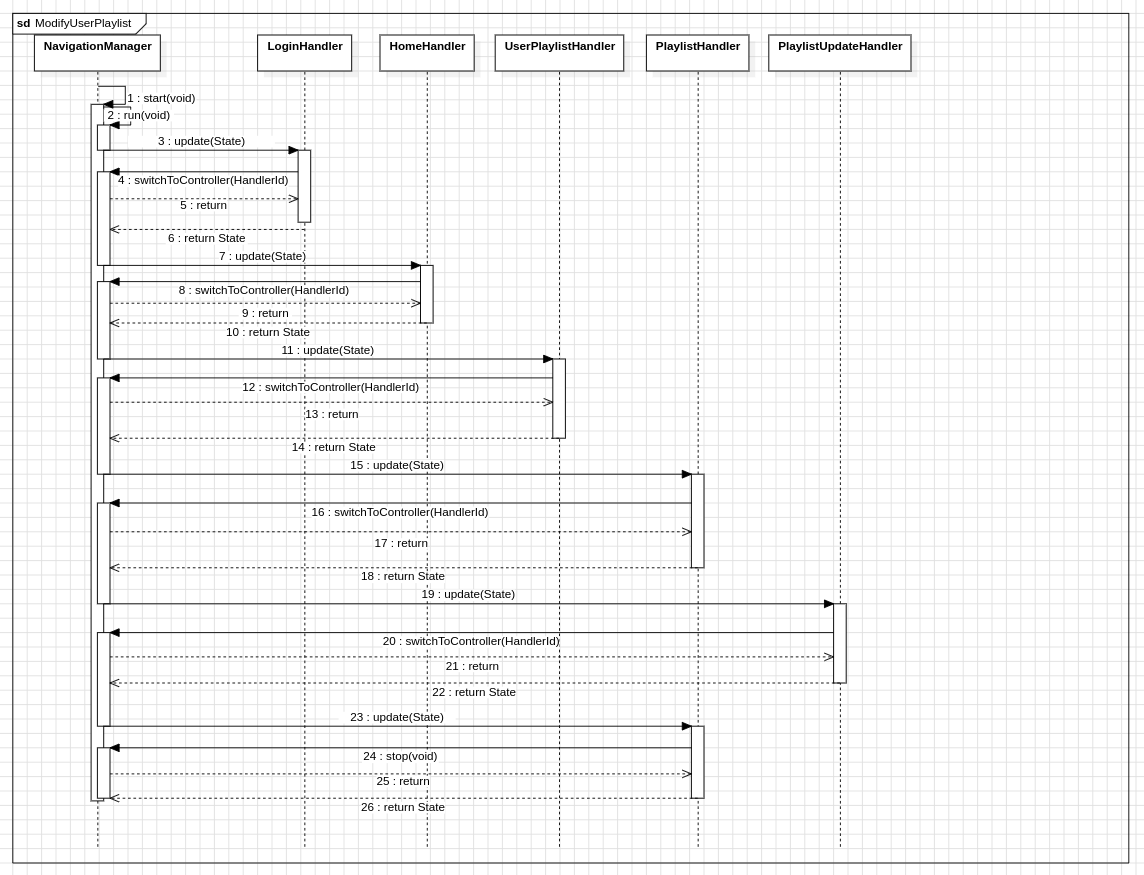
\includegraphics[scale=0.30]{sequenze01}
\end{figure}

\section{Scelte di progetto}

Abbiamo scelto di strutturare il progetto creando una divisione tra domain model, business logic e data
access objects.
\begin{itemize}
  \item
    Il package  \textbf{domainmodel} definisce le classi che simboleggiano gli elementi con cui l'utente
    interagisce.
  \item
    il package \textbf{businesslogic} descrive le modalità e le possibilità di interazione che l'utente
    ha con tali oggetti.
  \item
    il \textbf{dao} garantisce la persistenza di alcuni oggetti all'interno dell'applicazione.

   \end{itemize}
    
\section{Documentazione}
   
\subsection{Domain model}

\begin{figure}[H]
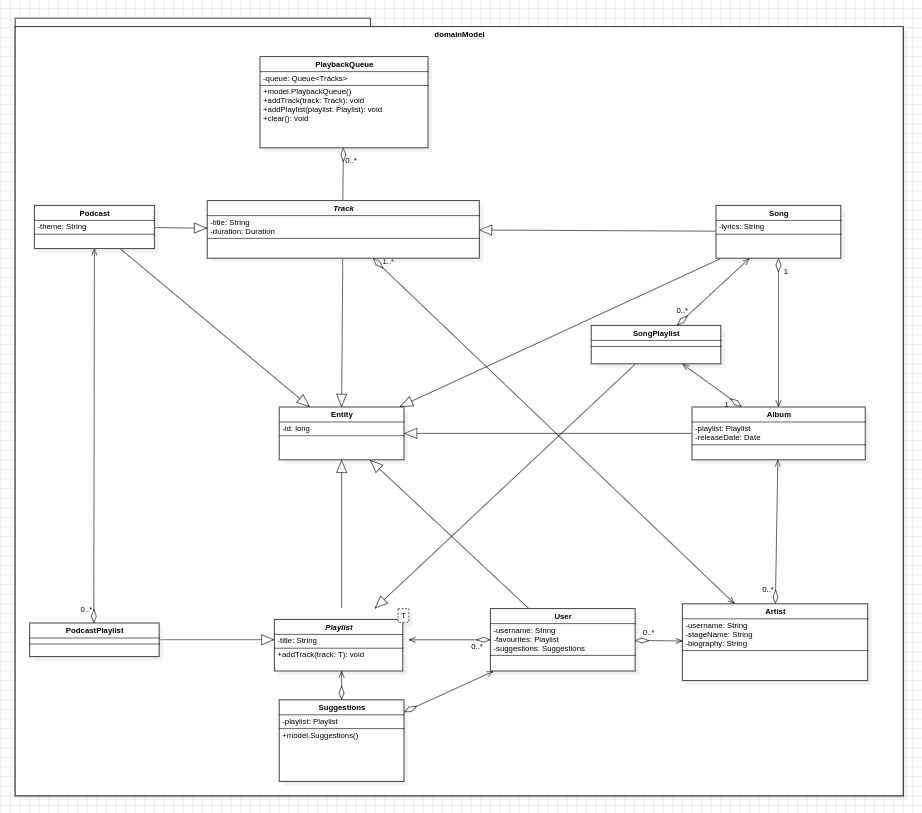
\includegraphics[scale=0.4]{model01}
\end{figure}

\subsubsection{Entity}
Classe base astratta che garantisce la presenza di un ID al fine di localizzare gli oggetti nel database.
\subsubsection{Customer}
Rappresenta il cliente e contiene le sue credenziali di accesso oltre alle playlist salvate. 
\subsubsection{Artist}
Rappresenta l'artista e contiene le sue credenziali d'accesso e gli album da lui caricati.
\subsubsection{Track}
Rappresenta un qualsiasi oggetto che può essere aggiunto alla coda\\ di riproduzione.
\subsubsection{Song}
Concretizzazione di Track che rappresenta una canzone.
\subsubsection{Podcast}
Concretizzazione di Track che rappresenta un podcast.
\subsubsection{Playlist}
Rappresenta una playlist ed espone i metodi per aggiungere o rimuovere\\ delle track in testa oppure in coda.
\subsubsection{Album}
Permette all'utente di riprodurre le canzoni al suo interno ma è immutabile.
\subsubsection{Suggestion}
Rappresenta il possibile interesse del cliente verso una track.
\subsubsection{PlaybackQueue}
Rappresenta la coda di riproduzione e permette di aggiungere in testa ed in coda oltre ad eliminare in testa.



\subsection{Business logic}

\begin{figure}[H]
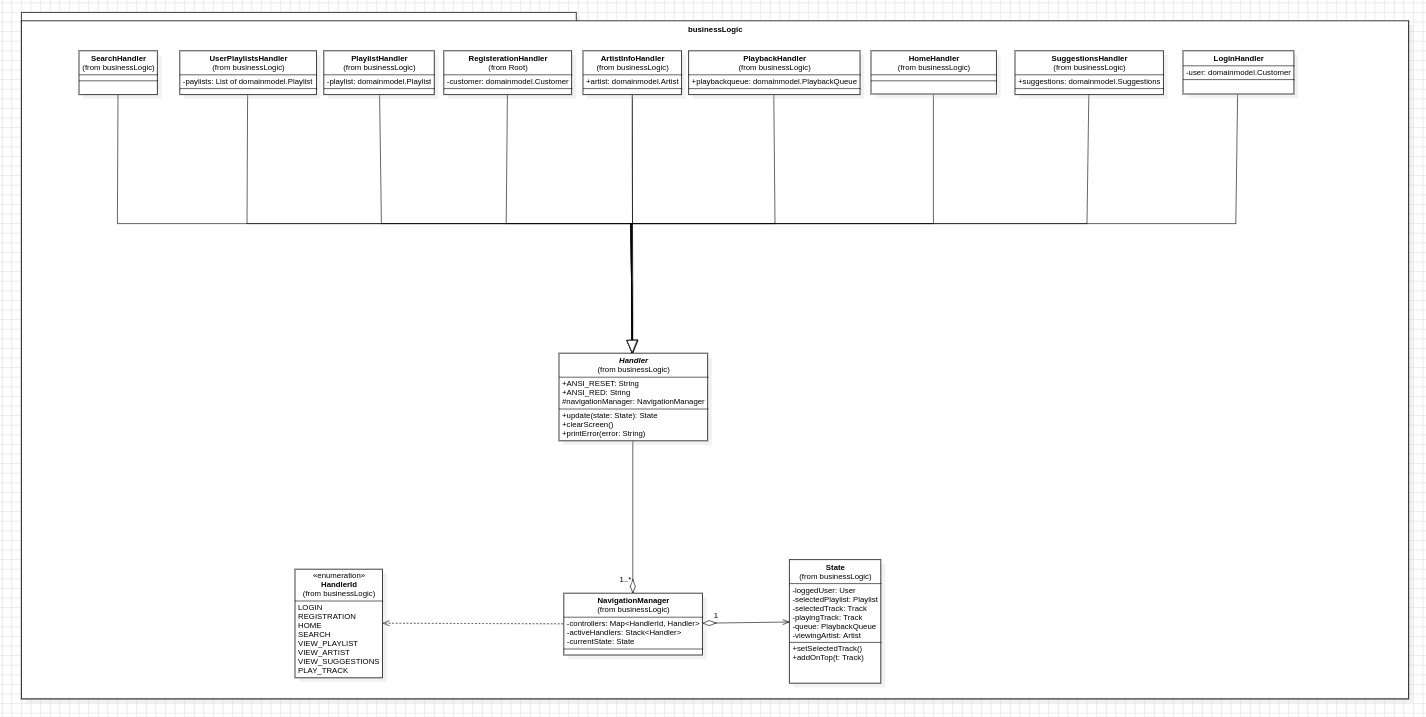
\includegraphics[scale=0.28]{logic01}
\end{figure}

\subsubsection{Handler}
Classe base astratta che rappresenta un handler generico.\\
Essa garantisce la presenza di un metodo update in ogni handler che contiene la logica di quest'ultimo.
\subsubsection{State}
Classe che permette ai vari handler di comunicare tra loro dati come
l'utente loggato, la canzone o la playlist selezionata
\subsubsection{NavigationManager}
Gestisce la navigazione tra le pagine passando il controllo ai vari handler.
\subsubsection{AlbumsHandler}
Permette di visualizzare o riprodurre un album.
\subsubsection{ArtistInfoHandler}
Mostra le informazioni salienti di un artista.
\subsubsection{HomeHandler}
Contiene la schermata di ingresso e instrada l'utente verso le varie pagine.
\subsubsection{LoginHandler}
Permette all'utente di effettuare l'accesso con un nome utente e una password o
eventualmente passare alla schermata di registrazione.
\subsubsection{PlaybackHandler}
Gestisce la coda di riproduzione e permette all'utente di visualizzare i
brani contenuti in essa.
\subsubsection{PlaylistHandler}
Mostra all'utente i brani contenuti in una data playlist e permette ad esso di
aggiungerla alla coda di riproduzione.
\subsubsection{RegistrationHandler}
Permette all'utente di registrarsi all'interno dell'applicazione con un
nome utente ed una password.
\subsubsection{SearchHandler}
Gestisce la ricerca all'interno delle canzoni, dei podcast e degli artisti disponibili.
\subsubsection{SuggestionsHandler}
Mostra all'utente le track suggerite dall'applicazione.
\subsubsection{UserPlaylistsHandler}
Mostra l'elenco delle playlist create dall'utente.

\subsection{Dao}

\begin{figure}[H]
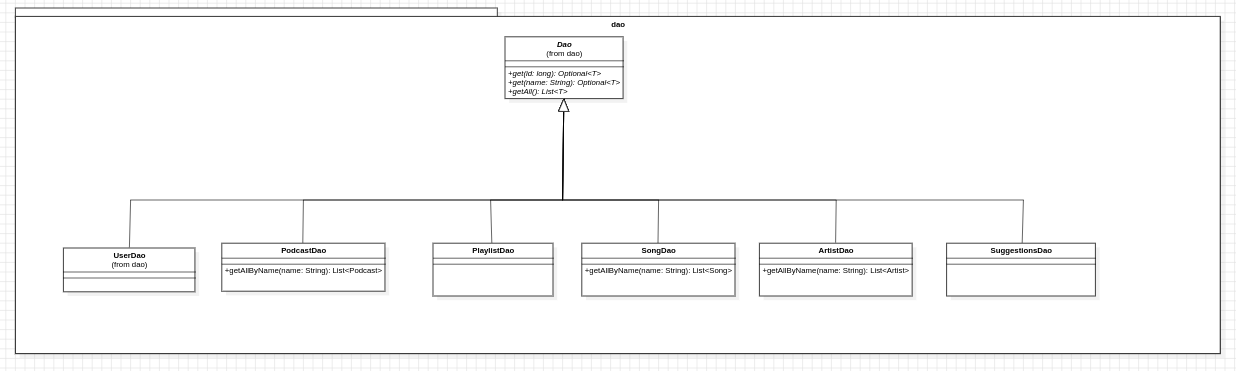
\includegraphics[scale=0.3]{dao01}
\end{figure}

\subsubsection{Dao}
Classe base astratta del data acces object che garantisce la capacità di leggere
o scrivere oggetti dal database.
\subsubsection{CustomerDao}
Permette di ottenere oggetti Customer dal database a patire dal loro nome utente o ID.
\subsubsection{ArtistDao}
Permette di ottenere oggetti Artist dal database a patire dal loro nome utente o ID.
\subsubsection{SongDao}
Permette di ottenere oggetti Song dal database in base ad una parola chiave.
\subsubsection{PodcastDao}
Permette di ottenere oggetti Podcast  dal database in base ad una parola chiave.
\subsubsection{PlaylistDao}
Permette di leggere e scivere le playlist dell'utente dal database.
\section{Test effettuati}   
\end{document}
